% ============================================================
% LLM-BLM プロジェクト総合報告書 3（2026-10-18 夜〜25）
% コンパイル：tectonic -X compile LLM-BLM_総合報告書3.tex   （XeTeX 系。このフォルダで実行する）
% 図は LLM-BLM_総合報告書3_図/ にある。どれも各実験の報告書の図の写し（元の場所は図の注に書いた）。
% 第 VI 部「証明」は、やること.md の G1〜G6 を行った後に書き足す。
% ============================================================
\documentclass[xelatex,ja=standard,jafont=haranoaji,a4paper,10pt]{bxjsreport}
\setpagelayout*{left=25mm,right=25mm,top=28mm,bottom=28mm,footskip=12mm}

\usepackage{amsmath,amssymb}
\usepackage{booktabs,longtable,array,multirow}
\usepackage{graphicx}
\usepackage{adjustbox}
\usepackage{xcolor}
\usepackage{tikz}
\usetikzlibrary{arrows.meta,positioning,calc,fit}
\usepackage{enumitem}
\usepackage{caption}
\usepackage{float}
\usepackage[most]{tcolorbox}
\usepackage[hidelinks,bookmarksnumbered]{hyperref}
\pdfstringdefDisableCommands{\def\Omega{Ω}\def\Sigma{Σ}\def\SP{S&P500}\def\code#1{#1}}

\graphicspath{{LLM-BLM_総合報告書3_図/}}

\definecolor{c1}{HTML}{2A78D6}
\definecolor{c2}{HTML}{EB6834}
\definecolor{c3}{HTML}{1BAF7A}
\definecolor{c4}{HTML}{EDA100}
\definecolor{c7}{HTML}{6250D6}
\definecolor{ink2}{HTML}{52514E}
\definecolor{soft1}{HTML}{E4EEF9}
\definecolor{soft2}{HTML}{FBEEDF}
\definecolor{soft3}{HTML}{E3F3E9}
\definecolor{soft4}{HTML}{EEE8FA}
\definecolor{soft5}{HTML}{FBE6E6}

\newcommand{\SP}{S\&P500}
\newcommand{\code}[1]{\texttt{#1}}
\newcommand{\figref}[1]{図~\ref{#1}}
\newcommand{\tabref}[1]{表~\ref{#1}}
\newcommand{\chapref}[1]{第~\ref{#1}~章}
\newcommand{\secref}[1]{\ref{#1}~節}

\setlist[itemize]{leftmargin=1.6em,itemsep=0.2em,topsep=0.4em}
\setlist[enumerate]{leftmargin=1.8em,itemsep=0.2em,topsep=0.4em}

\captionsetup{font=small,labelfont=bf,skip=6pt}
\renewcommand{\arraystretch}{1.25}
\setlength{\LTpre}{6pt}
\setlength{\LTpost}{6pt}

\newtcolorbox{keybox}[1][要点]{enhanced,breakable,colback=soft1,colframe=c1,boxrule=0.5pt,arc=2pt,
  left=8pt,right=8pt,top=6pt,bottom=6pt,title={#1},fonttitle=\sffamily\bfseries\small,coltitle=white}
\newtcolorbox{notebox}[1][注意]{enhanced,breakable,colback=soft2,colframe=c2,boxrule=0.5pt,arc=2pt,
  left=8pt,right=8pt,top=6pt,bottom=6pt,title={#1},fonttitle=\sffamily\bfseries\small,coltitle=white}
\newtcolorbox{verdict}[1][判定]{enhanced,breakable,colback=soft4,colframe=c7,boxrule=0.5pt,arc=2pt,
  left=8pt,right=8pt,top=6pt,bottom=6pt,title={#1},fonttitle=\sffamily\bfseries\small,coltitle=white}

\tikzset{
  box/.style={draw=#1,fill=#1!12,rounded corners=2pt,align=center,inner sep=5pt,font=\small,minimum height=9mm},
  box/.default=c1,
  arr/.style={-{Stealth[length=2mm]},line width=0.6pt,color=ink2},
  lab/.style={font=\scriptsize,color=ink2}
}

\begin{document}

\hypersetup{pdftitle={LLM-BLM プロジェクト総合報告書 3},pdfauthor={小嶋 一輝},pageanchor=false}
\begin{titlepage}
\centering
\vspace*{30mm}
{\sffamily\Large 情報工学工房　プロジェクト総合報告書 3\par}
\vspace{14mm}
{\sffamily\bfseries\huge 大型株の当日の反応から、\par\vspace{3mm}小型株のドリフトと BLM へ\par}
\vspace{12mm}
{\large 大型株での実験 3〜11、補足実験 X02〜X05、\par\vspace{2mm}小型株の実験 S1〜S4、新しい 1,000 社での再現（R1）の記録\par}
\vspace{30mm}
{\large 電気通信大学　情報理工学域 III 類\par}
\vspace{3mm}
{\Large 小嶋 一輝\par}
\vspace{20mm}
{\large 2026 年 10 月 25 日 版\par}
\vfill
{\small 総合報告書 2（2026 年 10 月 18 日 版）の続き。対象は、総合報告書 2 に入っていない実験 3 以降の作業（2026 年 10 月 18〜25 日）。\par
\small 第 VI 部（BLM が効くことの証明）は、計画した確かめ（G1〜G6）を行った後に書き足す。\par}
\end{titlepage}
\hypersetup{pageanchor=true}

% ============================================================
% 概要
% ============================================================
\chapter*{概要}
\addcontentsline{toc}{chapter}{概要}

本書は、総合報告書 2（2026 年 10 月 18 日 版）に入っていない実験 3 以降の作業（10 月 18〜25 日）をまとめたものである。総合報告書 2 は、「LLM は決算発表文を読めるが、その情報は発表の 2 日のうちに株価に入る」ことを、事前登録した実験 2 で示した。本書の作業は 4 つに分かれる。

\begin{enumerate}
\item \textbf{大型株（\SP{}）での確かめ（実験 3〜11、X02〜X05）}：LLM の読み取りが、アナリスト予想・追加学習した FinBERT・先読みのない ChronoGPT を超えて反応を説明するかを確かめた。あわせて、読めた情報で月次・日次の BLM が時価総額加重を上回るか、TE の約束が守れるかを調べた。
\item \textbf{小型株への移動（実験 S1〜S4）}：大型株では情報が当日に入りきるので、注目が少なく発表の後も値がゆっくり動くと言われる小型株に移った。SEC のデータだけで、後で消えた会社も含む Russell 2000 に似た範囲を作り、1,000 社で事前登録した実験を 4 つ行った。
\item \textbf{新しい 1,000 社での再現（実験 R1）}：S1〜S4 を、重なりのない別の 1,000 社で 1 回ずつやり直し、BLM が比べる相手を上回るかを新しく事前登録して検定した。
\item \textbf{今どこまで言えるかの整理}：結果の確かさを段階に分け、「BLM で使える」と言うために足りない確かめ（G1〜G6）を計画した。
\end{enumerate}

\begin{keybox}[本書の主な結論]
\begin{itemize}
\item \textbf{大型株では、LLM の読み取りは本物だが、運用には使えなかった。}gpt-4o-mini の点数は、アナリスト予想（+116bp）、追加学習した FinBERT（+102bp）を統制しても反応を説明し、先読みのない ChronoGPT も従来の NLP を超えた（+34bp、$t$ 4.8）。しかし発表の翌日以降には情報が残らず（day 1 は +3.6bp）、月次の BLM は費用の後で時価総額加重を上回らなかった（約 10 年で月 +0.003\%）。
\item \textbf{小型株では、決算発表文の読み取りが、発表後 2〜60 日のドリフトを予測する（S1、事前登録した検定で支持）。}ChronoGPT＋リッジの点数が 1 標準偏差高いと、ドリフトは +76bp（$t$ 3.20、置換 $p$ 0.001）。発表後の変動率も、過去の変動率を超えて予測した（S2、支持）。
\item \textbf{この 2 つは、新しい 1,000 社でも再現した（R1）。}S1 は +54bp（$t$ 2.22、置換 $p$ 0.008）、S2 は +1.1\%（$t$ 3.0）。S3（文章のリスクの点数で共分散を補正しても TE は正確にならない）も同じく効果がなかった。S4（TE の上限の校正）は再現しなかった。
\item \textbf{BLM は、株価の誤りを除くと、両方の標本で比べる相手を年約 3\% 上回った。ただしこれは探索の結果である。}事前登録した R-BLM の検定は「支持」（年 +5.3\%）だったが、その約半分は yfinance の株価の誤り 1 日（破産から再出発した会社の古い株と新しい株のつなぎ、+25,700\%）による上乗せで、実現の TE も約束の約 3 倍（10.0\%）だった。誤りを除くと年 +2.9\%（95\% 区間 +1.0〜+4.8\%、TE 3.2\%、情報レシオ 0.89）、元の標本では +3.0\%（TE 3.1\%）。
\item \textbf{したがって、「LLM の読み取りに予測力がある」はほぼ確かめられたが、「BLM で使える」はまだ証明していない。}足りないのは、偽のビューとの比較、ファクターでの説明、誤りを除く規則を先に固定した事前登録の検定、生存者バイアス・費用・容量の確認である（\chapref{ch:plan}）。
\end{itemize}
\end{keybox}

本書の数値は、とくに断りがなければ、リポジトリのブランチ \code{feature/earnings-events} の \code{experiments/*/results/} の結果のファイルから取った。各実験の詳しい報告は、\code{資料集/02\_実験/} の報告書にある（付録~\ref{app:docs}）。

\setcounter{tocdepth}{1}
\tableofcontents

% ============================================================
\part{背景}
% ============================================================

\chapter{総合報告書 2 の後に残っていた問い}\label{ch:intro}

総合報告書 2 の結論は、次の 3 つだった。

\begin{enumerate}
\item LLM に数値のリターンを予想させても価値はない（H01〜H07）。
\item LLM が決算発表文から読み取った点数は、発表をはさむ 2 取引日の超過リターンを説明する（実験 2、1 標準偏差あたり +120bp、$t$ 9.4）。
\item しかし反応は 2 日のうちに出尽くし、その後のドリフトは有意でない。
\end{enumerate}

ここから、次の問いが残った。

\begin{keybox}[本書で答える問い]
\begin{enumerate}
\item \textbf{LLM の読み取りは本物か。}アナリスト予想、反応で学習させた専用のモデル、先読みのない LLM と比べても残るか（\chapref{ch:large-read}）。
\item \textbf{読めた情報で運用できるか。}発表の翌日、月次、日次の BLM で、費用の後に時価総額加重を上回るか。BLM の TE の約束は守れるか（\chapref{ch:large-blm}）。
\item \textbf{情報がゆっくり入る市場ならどうか。}注目の少ない小型株で、読み取りは発表の後のドリフトを予測するか。それを BLM に入れると、比べる相手に勝てるか（第 III〜V 部）。
\item \textbf{どこまで言い切れるか。}結果は別の会社でも再現するか。「BLM で使える」と言うには何が足りないか（\chapref{ch:status}、\chapref{ch:plan}）。
\end{enumerate}
\end{keybox}

本書でも、総合報告書 2 と同じく、株価の反応を計算する前に計画と評価のコードを同じコミットで固定し、1 回だけ実行する\textbf{事前登録}の方式を使った。結果を見た後の分析は、すべて「探索」と明記した。

% ============================================================
\part{大型株の決算発表（実験 3〜11、X02〜X05）}
% ============================================================

\chapter{LLM の読み取りは本物か}\label{ch:large-read}

対象は \SP{} の構成銘柄の決算発表（8-K の Item 2.02 に付いた発表文）、目的変数は発表をはさむ 2 取引日の、セクターの ETF との差の超過リターンである。どの実験も、総合報告書 2 の実験 2 と同じ統制（数値の驚き、辞書、FinBERT、TF-IDF＋リッジ、発表前のリターン、規模、固定効果）を入れた。

\section{統制を強めても残る}

\begin{longtable}{p{6.2cm}p{2.6cm}p{5.0cm}}
\caption{gpt-4o-mini の点数の係数（1 標準偏差あたり）。統制を足していっても、ほとんど小さくならない。}\label{tab:controls}\\
\toprule
\textbf{統制に加えたもの} & \textbf{LLM の係数} & \textbf{実験} \\
\midrule
\endfirsthead
\toprule
\textbf{統制に加えたもの} & \textbf{LLM の係数} & \textbf{実験} \\
\midrule
\endhead
\bottomrule
\endfoot
実験 2 の統制 & +120bp（$t$ 9.4） & 実験 2（総合報告書 2） \\
＋アナリスト予想との差（EPS） & +116bp（$t$ 9.4） & 実験 3。係数の 97\% が残った \\
＋反応で追加学習した FinBERT & +102bp（$t$ 7.8） & 実験 4。FinBERT 自身は +71bp。説明力は LLM が約 2.4 倍 \\
＋ChronoGPT の埋め込み＋リッジ & +112bp（$t$ 8.9） & 実験 5 \\
＋ChronoGPT の LoRA & +117bp & 実験 10 \\
\end{longtable}

\section{先読みのない LLM でも読める}

gpt-4o-mini は評価の期間の株価を知っているおそれがある（先読み）。そこで、2015 年までの文章だけで学習した ChronoGPT（版 2015、1.55B）の最後の層のベクトルを取り出し、その時点より前の発表だけで学習したリッジ回帰で反応を予測した（He ほか 2025 の方法）。

\begin{itemize}
\item 実験 5（2016〜2023 年）：+34bp（$t$ 5.5）。TF-IDF の効果を吸収した。
\item 実験 11（2020 年以降、事前登録した最後の比較）：数値の統制と NLP 3 つを超えて +34bp（$t$ 4.8）。3 通りの期間の切り方のすべてで支持。
\item 実験 10（ChronoGPT を反応で LoRA の追加学習、約 7.6 時間）：線形のリッジより弱かった（説明力の増分 +0.13 ポイント）。学習の損失はほとんど下がらなかった。
\end{itemize}

実験 11 では、文章の掃除、読む範囲、セクターへのまとめ方、埋め込みの取り方、圧縮（LLMLingua）の 5 つの修正を、開発の期間の機械的な規則で試したが、主な切り方では残った修正はなかった。探索で、ChronoGPT の真ん中の層（52 層のうち 26 層目）の埋め込みが説明力を約 1.6 倍にした（増分 0.49 → 0.80）。この「真ん中の層」は、小型株の副次の点数（\code{chrono\_mid\_ridge}）として使った。

\begin{keybox}
LLM の読み取りは、アナリスト予想・専用に学習したモデル・先読みのない LLM のどれと比べても残る。「gpt-4o-mini が答えを覚えていただけ」ではない。
\end{keybox}

\chapter{読めた情報で運用できるか}\label{ch:large-blm}

\section{情報はいつまで残るか（実験 8）}

発表の翌日（day 1）の超過リターンは +3.6bp（$t$ 0.93）で、95\% 区間の上限でも +11bp だった。2 日の反応（約 +100bp）のほとんどは発表の当日に出る。day 2〜21 のドリフトも +10bp（$t$ 0.83、実験 2）。日次の BLM は回転率が 1 日 42\% になり、費用の後で年 $-20\%$ だった。

\section{月次の BLM（実験 7・9）}

\begin{itemize}
\item 実験 7（gpt-4o-mini、2024-01〜2026-07 の 31 か月）：時価総額加重に月 +0.10\%（$t$ 1.22）、支持されない。点数を銘柄の間で混ぜた対照には月 +0.20\%（$t$ 2.30、副次）。
\item 実験 9（ChronoGPT、約 10 年）：月 +0.003\%（$t$ 0.04）。混ぜた対照には +0.15\%（$t$ 1.78）。
\end{itemize}

点数の中身に弱い価値は残っているかもしれないが、比率を動かす費用を払うと消える大きさだった。

\section{TE の約束（X02〜X05）}

BLM は事前の TE を 3\% 以下にして最適化したが、実際の TE は約 1.5 倍になった（X01）。

\begin{longtable}{p{2.0cm}p{5.4cm}p{6.4cm}}
\caption{TE のずれを直す試み。}\label{tab:te}\\
\toprule
\textbf{実験} & \textbf{やったこと} & \textbf{結果} \\
\midrule
\endfirsthead
\bottomrule
\endfoot
X02 & 共分散の窓、EWMA の半減期 & ewma126 で 4.58\% → 4.26\%。それでも目標の 1.42 倍。窓では直らない \\
X03 & 過去 36 か月の「実現 ÷ 目標」で上限を割る（校正） & 4.79\% → 3.38\%（ewma126 と合わせて 3.28\%）。ずれは半分以下 \\
X04 & VIX で共分散の大きさを合わせる & 支持されない。VIX は市場全体のぶれで、銘柄の間のばらつきは捉えきれない \\
X05（探索） & 見通しの $\alpha$ に倍率を掛ける & 実験 7・9 の $\alpha$ は、持つ期間に合った大きさの $\sqrt{21}\approx 4.6$ 倍だった（日次の $\sigma$ のまま 1 か月持った）。倍率 0.03 以上では TE の上限が毎月効き、結果はまったく同じ \\
\end{longtable}

X03 の校正は小型株の S4 に、X05 の「$\alpha$ を持つ期間に合わせる」は小型株の BLM のビュー（$q = \pi + \mathrm{IC}\cdot\sigma\cdot z/\sqrt{h}$、$h$ は持つ日数）に引き継いだ。

\chapter{方針の転換：小型株へ}\label{ch:pivot}

\section{なぜ小型株か}

大型株では、LLM が読める情報は、市場も発表の当日に読んでいた。BLM のビューが価値を持つには、判断の時点でまだ価格に入っていない情報が要る。決算発表の後のドリフト（PEAD、Bernard・Thomas 1989）は、大型株では 2006 年以降ほぼ消えたと報告されている（Martineau 2022）。一方で、アナリストや投資家の注目が少ない小さな会社では、悪いニュースほどゆっくり価格に入るという報告がある（Hong・Lim・Stein 2000）。そこで、同じ読み取りを小型株に当てることにした。

\section{ヘッジファンドの手法の調査}

方針を決める前に、ヘッジファンドの投資手法の研究を、切り口を変えて Gemini Deep Research に 3 回調べさせ、挙がった文献を照合して報告書（約 110 ページ、\code{資料集/05\_解説/ヘッジファンドの投資手法/}）にまとめた。挙がった 209 本の題名のうち 189 本は機械的な照合で一致し、残りの 20 本も Crossref で 1 本ずつ手で確かめた。

この調査から、次の 3 点を小型株の設計に取り入れた。

\begin{itemize}
\item \textbf{速いシグナルを遅い売買で使うと価値が消える}。小型株でも、ドリフトの期間（発表後 2〜60 日）に合わせて持つ。
\item \textbf{小型株では費用が成績を決める}（Chordia ほか 2009）。費用は片道 0.3\% とし、0\%・0.5\% も並べる。
\item \textbf{公表されたシグナルは減衰し、試した数が多いほど見かけの成果が出る}。事前登録と、判定に使う検定の数の制限を続ける。
\end{itemize}

% ============================================================
\part{小型株（実験 S1〜S4）}
% ============================================================

\chapter{小型株のデータ}\label{ch:scdata}

\section{範囲の作り方}

指数会社の構成銘柄の履歴は有料なので、SEC のデータだけで Russell 2000 に似た範囲を作った。

\begin{enumerate}
\item 2015〜2025 年の各年について、XBRL の frames から、全提出者の浮動株時価総額（\code{dei:}\allowbreak\code{EntityPublicFloat}）を取った（会社・年で 64,269 件）。100 万ドル未満、4 兆ドル超、同じ会社のほかの年から 200 倍以上ずれる値は使わない。
\item 米国に所在する提出者の中で並べ、1,001〜3,000 位を小型株の範囲とした（おおむね 1 億〜40 億ドル）。範囲に一度でも入った会社は 4,921 社で、後で消えた会社も入る。
\item 発表の時点の範囲には、その日に分かっていた最新の浮動株時価総額（測った日から 9 か月後に使い、21 か月より古いものは使わない）を使う。
\end{enumerate}

\section{生存者バイアス}

株価は yfinance から取るので、今のティッカーで株価がない会社は使えない。範囲に入った会社・年のうち、決算の 8-K を出した 20,282 件の 31.7\% が欠け、2015 年は半分が欠けた（\figref{fig:coverage}）。消えた 1,826 社の 79\% は買収、15\% は倒産だった。

\begin{figure}[H]
\centering
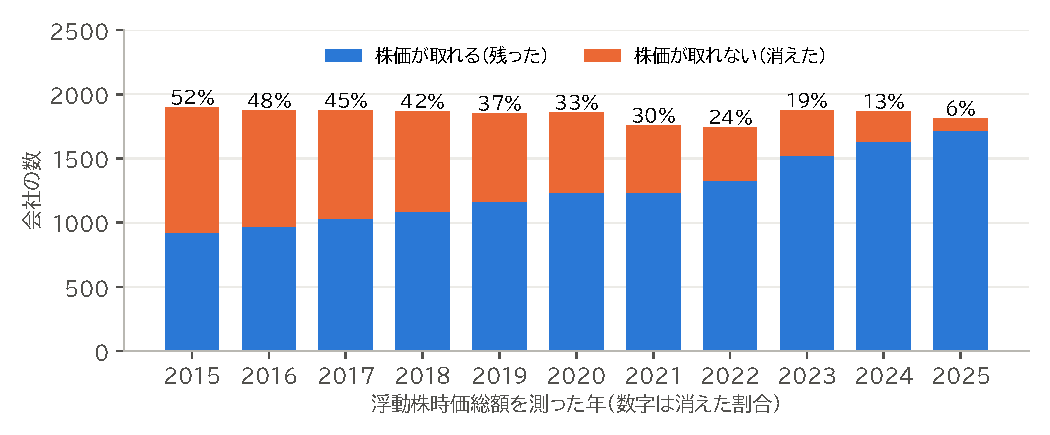
\includegraphics[width=0.85\linewidth]{sc_coverage.pdf}
\caption{小型株の範囲に入った会社（決算の 8-K を出したもの）のうち、株価が取れる会社と取れない会社（『小型株のデータ』の図）。}
\label{fig:coverage}
\end{figure}

\section{標本}

範囲に一度は入り、今の株価があり、2016 年以降の決算の 8-K が 4 本以上ある 2,400 社から、1,000 社を乱数の種 0 で選んだ（元の標本）。決算発表文、財務データ（EPS・売上の前年同期との差による驚き）、点数（辞書、FinBERT、FinBERT の追加学習、ChronoGPT の埋め込み＋リッジ、gpt-4o-mini）は、大型株と同じコードで作った。

\chapter{S1：読み取りはドリフトを予測するか}\label{ch:s1}

\begin{verdict}[S1 の主な検定（事前登録）：支持]
$\text{ドリフト}_{2\text{〜}60} = \beta\cdot\text{chrono\_ridge} + \text{統制} + \text{業種} + \text{四半期} + \varepsilon$。2020 年以降に範囲の中で出た発表 15,174 件、反応の日 1,384 日（反応の日でクラスターした標準誤差）。

$\beta$ = +76.1bp/SD（95\% 区間 +29.5〜+122.6）、$t$ 3.20、置換（1,000 回）の片側 $p$ 0.001。
\end{verdict}

統制は、数値の驚き（SUE、売上）、欠けの印、発表前 1 か月のリターン、規模、2 日の反応そのものである。2 日の反応を統制しているので、この係数は「発表の当日に市場が読んだ分」を除いた、その後の動きの予測である。

\begin{itemize}
\item 2〜21 日ではほぼゼロ（$t$ 0.13）で、ドリフトは主に 22〜60 日目に出る（探索：22〜60 日だけで +70.8bp、$t$ 3.82）。
\item 探索で過去 1 年のモメンタムを統制に足しても消えなかった（+92.5bp、$t$ 3.81）。規模の小さい半分（+81.3bp）でも大きい半分（+66.7bp）でも出た。
\item gpt-4o-mini（2024 年以降、副次）：+148.9bp（$t$ 4.21）。
\item ドリフトを正解に学習したリッジ（事前登録した探索）は予測しなかった（$-3.1$bp）。反応で学習した点数のほうが、ドリフトを当てる。
\end{itemize}

\begin{figure}[H]
\centering
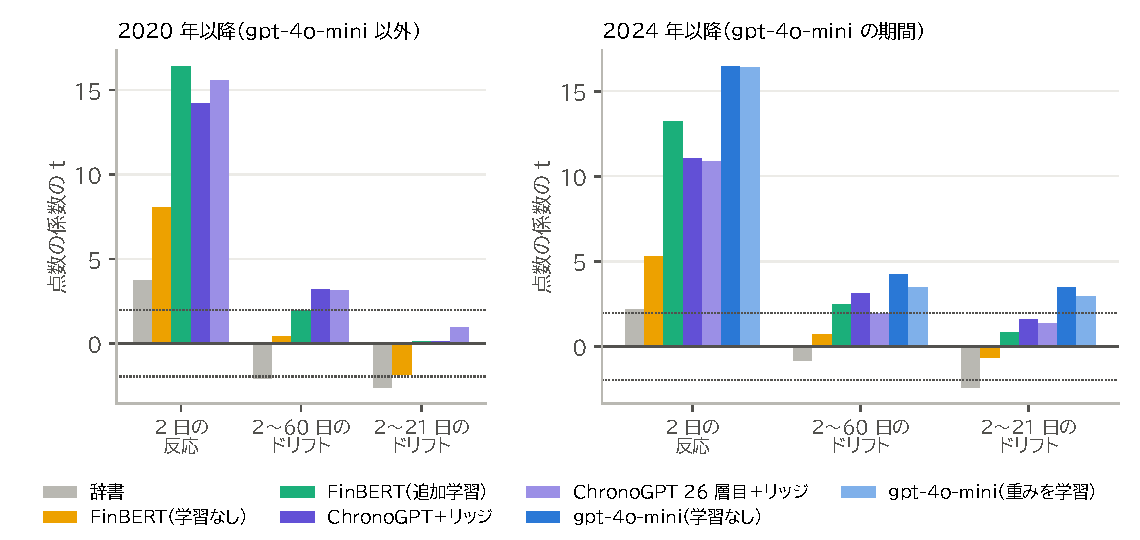
\includegraphics[width=0.85\linewidth]{s1_compare.pdf}
\caption{S1 の点数ごとの係数の $t$。点線は $\pm 1.96$（『実験 S1』の図）。}
\label{fig:s1compare}
\end{figure}

\begin{notebox}[単純なポートフォリオでは有意にならない]
\code{chrono\_ridge} の上位 20\% を浮動株時価総額で加重した月次のポートフォリオと、範囲の全社の浮動株時価総額加重を比べると、費用 0.3\% の後で月 +0.16\%（Newey--West の $t$ 0.73、80 か月）で有意ではなかった（\figref{fig:s1portfolio}）。回帰では効くのに単純な組み方では出ない理由は、まだ説明できていない（\chapref{ch:plan} の G6）。
\end{notebox}

\begin{figure}[H]
\centering
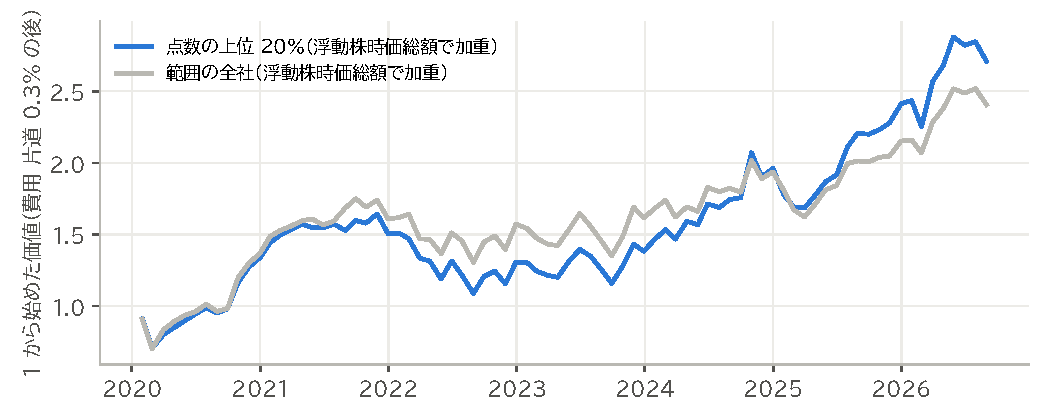
\includegraphics[width=0.85\linewidth]{s1_portfolio.pdf}
\caption{ChronoGPT＋リッジの上位 20\% と範囲の全社（2020 年 1 月を 1、片道 0.3\% の費用の後。『実験 S1』の図）。}
\label{fig:s1portfolio}
\end{figure}

\chapter{S2：読み取りは変動率を予測するか}\label{ch:s2}

\begin{verdict}[S2 の主な検定（事前登録）：支持]
ChronoGPT のベクトルで「発表後の変動率 − 発表前の変動率」を学習した四半期ごとのリッジの点数（\code{chrono\_risk}）は、過去の変動率（発表前 60 日、その前の 1 年）・規模・驚きの大きさ・反応の大きさを統制しても、発表後 2〜60 日の変動率を予測した。

1 標準偏差あたり +1.51\%（変動率の対数 × 100、95\% 区間 +0.77〜+2.25）、$t$ 4.01、置換の片側 $p$ 0.001。
\end{verdict}

ただし、決定係数の増分は 0.036 ポイントと小さく、標本外で変動率の水準を予測すると、点数を足した方がわずかに悪かった（二乗誤差の比 1.011）。点数が持っているのは、同じ時期の銘柄の間の相対的なリスクの情報で、水準を当てる力ではない。

\chapter{S3・S4：BLM のリスクを正しくする}\label{ch:s34}

\section{小型株の BLM}

S1 の点数を BLM のビューにして、範囲の中の標本の会社で運用した。

\begin{itemize}
\item 組み直しは 2015 年末か 2023 年末から、四半期・半年・1 年ごと。次の組み直しまで持つ。
\item 共分散は直近 252 日の Ledoit--Wolf、市場の比率は浮動株時価総額。均衡のリターンは $\pi = \delta\Sigma w_{\mathrm{mkt}}$（$\delta = 2.5$）。
\item ビューは、直近 92 日以内に発表がある銘柄に 1 本ずつ：$q = \pi + \mathrm{IC}\cdot\sigma\cdot z/\sqrt{h}$（$z$ は点数の順位の正規点数、$\mathrm{IC} = 0.05$、$h$ は持つ日数。Grinold 1994 の $\alpha$ を持つ期間に合わせた）。
\item $\Omega = \tau\,\mathrm{diag}(P\Sigma P^{\top})$（He・Litterman 1999）、$\tau = 0.025$。
\item ロングのみ、事前の TE 3\% 以下、費用は片道 0.3\%。比べる相手は、範囲の中の標本の会社の浮動株時価総額加重。
\end{itemize}

\section{S3：文章のリスクの点数で共分散を補正する}

S2 の結果から、発表後 60 日の銘柄の分散を補正した（$\Sigma' = S\Sigma S$、$s = \exp(\hat y - l)$ を $[0.5, 2]$ に切る）。物差しは $b = \sqrt{\overline{z^2}}$（$z$ = 日次の超過リターン ÷ 事前の TE。1 なら事前の TE が正確）である。

\begin{verdict}[S3 の主な検定（事前登録）：支持されない]
株価だけの補正（B）に文章のリスクの点数を足しても（C）、$b$ は 1.2199 → 1.2195 で、ほぼ変わらなかった（片側 $p$ 0.201）。一方、株価による補正そのものは、補正なし（A）の 1.254 を 1.220 に下げた（$p < 0.001$、副次）。
\end{verdict}

\section{S4：TE の上限を過去の偏りで校正する}

X03 と同じ考えで、上限を $L_d = \mathrm{clip}(3\%/b_{\mathrm{past}}, 1\%, 6\%)$ とした（$b_{\mathrm{past}}$ は判断の日より前の 756 日の偏り）。物差しは $g$ = 実現の TE ÷ 3\% である。

\begin{verdict}[S4 の主な検定（事前登録）：支持]
2017 年以降（2,449 日）、$g$ は 1.22 → 1.05（実現の TE 3.7\% → 3.2\%）、片側 $p$ 0.004。情報レシオはほぼ保たれた（1.01 → 0.96）。
\end{verdict}

\begin{figure}[H]
\centering
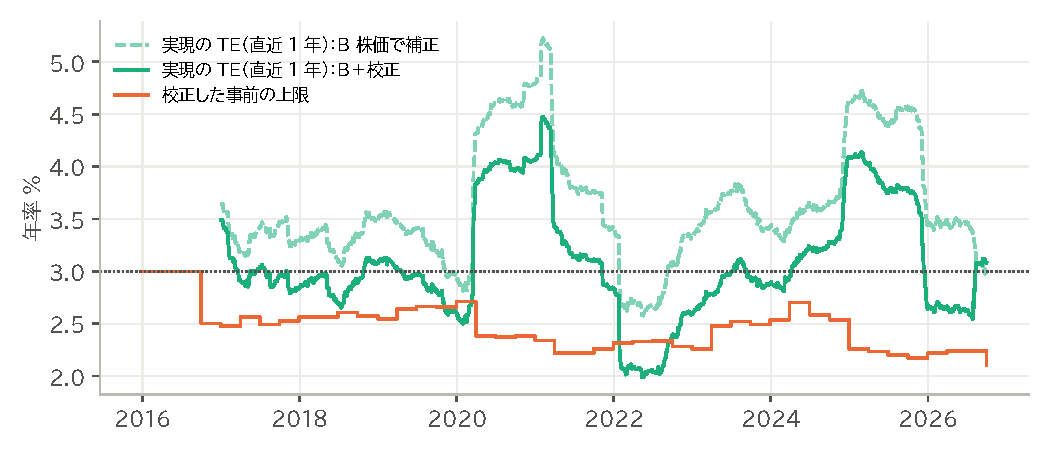
\includegraphics[width=0.85\linewidth]{s4_te.pdf}
\caption{直近 1 年の実現の TE（校正なしと校正あり）と、校正した事前の上限。点線は約束の 3\%（『実験 S4』の図）。}
\label{fig:s4te}
\end{figure}

この時点で、S4 の形の BLM（2015 年末から四半期ごと、ChronoGPT＋リッジ、共分散 B、校正あり）は、比べる相手を年 +3.0\% 上回っていた（TE 3.2\%）。ただしこれは検定していない数字で、S2〜S4 の設計は S1 の結果を見た後だった。そこで、別の会社で確かめることにした。

% ============================================================
\part{新しい 1,000 社での再現（実験 R1）}
% ============================================================

\chapter{再現の判定}\label{ch:r1}

\section{方法}

元の標本を選んだのと同じ条件を満たす 2,400 社のうち、元の 1,000 社を除いた 1,400 社から、1,000 社を乱数の種 1 で選んだ（重なり 0）。決算発表文 38,601 本の取得、点数付け（ChronoGPT と FinBERT は借りた GPU、gpt-4o-mini は 11,824 本で約 7 ドル）をした後、計画（\code{experiments/R1\_replication/preregistration.md}）とコードをコミット \code{161cab5} で固定し、S1〜S4 を元と同じ設定・同じ乱数の種で 1 回ずつ実行した。

S1・S2・S4 は元と同じ基準で「支持」なら「再現した」、元が「支持されない」だった S3 は再び「支持されない」なら「再現した（効果なし）」とした。

\section{結果}

\begin{table}[H]
\centering\small
\caption{元の 1,000 社と新しい 1,000 社の主な検定。}
\label{tab:r1}
\begin{tabular}{p{3.6cm}p{3.6cm}p{3.6cm}p{2.4cm}}
\toprule
実験 & 元の標本 & 新しい標本 & 判定 \\
\midrule
S1：ドリフト & +76.1bp/SD、$t$ 3.20、置換 $p$ 0.001 & +54.5bp/SD、$t$ 2.22、置換 $p$ 0.008 & \textbf{再現した} \\
S2：変動率 & +1.51\%/SD、$t$ 4.01 & +1.06\%/SD、$t$ 3.01 & \textbf{再現した} \\
S3：文章で共分散を補正 & $b$ 1.220 → 1.219、$p$ 0.201 & $b$ 3.552 → 3.494、$p$ 0.287 & 再現した（効果なし） \\
S4：TE の校正 & $g$ 1.22 → 1.05、$p$ 0.004 & $g$ 3.72 → 3.32、$p$ 0.148 & \textbf{再現しなかった} \\
\bottomrule
\end{tabular}
\end{table}

gpt-4o-mini（学習なし）のドリフトも、新しい標本で +83.9bp（$t$ 2.53）だった（元は +148.9bp、$t$ 4.21）。

\begin{figure}[H]
\centering
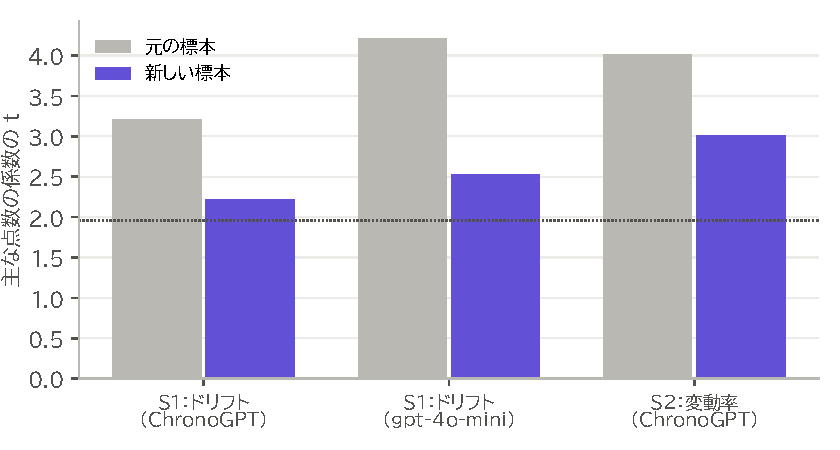
\includegraphics[width=0.7\linewidth]{r1_coef.pdf}
\caption{主な点数の係数の $t$、元と新しい標本。点線は 1.96（『実験 R1』の図）。}
\label{fig:r1coef}
\end{figure}

\chapter{R-BLM と株価データの誤り}\label{ch:rblm}

\section{事前登録した検定}

R1 では、新しい主な検定として次を事前登録した。S4 の形の BLM の、2017 年以降の日次の超過リターン（BLM − 比べる相手）の平均が正か。63 日の循環ブロック・ブートストラップ（Politis・Romano 1992）2,000 回で、片側 $p < 0.05$ なら支持。

\begin{verdict}[R-BLM（事前登録）：支持。ただし TE は約束の約 3 倍]
年 +5.3\%（日次の平均 × 252、95\% 区間 +1.1〜+12.2\%）、片側 $p < 0.001$。実現の TE は 10.0\%、情報レシオ 0.53。
\end{verdict}

\section{原因：破産からの再出発のつなぎ}

TE が約束の 3 倍になった理由を、結果を見た後に調べた（探索）。日々の超過リターンの 2 乗の合計の 93\% が、上位 5 日から来ていた（\figref{fig:r1active}）。最も大きい日は 2020-11-20 で、Oasis Petroleum（今の CHRD）の調整後終値が 0.07 → 18.8（約 +25,700\%）になっていた。この会社は 2020 年 11 月に破産の手続きから新しい株で再出発しており、yfinance が古い株と新しい株の価格をつないだものだった。古い株主が得たリターンではない。

この 1 日で BLM と相手の差が +30\% 開いた。S4 の校正は過去 756 日の偏りで上限を割るので、この日の後、2020-12〜2023-09 の 12 回の組み直しで上限が下限の 1\% に張り付いた。S4 が再現しなかったのも、主にこの誤りのためだった。

同じ種類の日は元の標本にもあった（AMPY 2016-10-24 の +16,079\% など）。2015 年以降の会社 × 日 2,953,000 のうち、+300\% 超は元 30・新 38、$-80\%$ 未満は元 30・新 31 だった。

\begin{figure}[H]
\centering
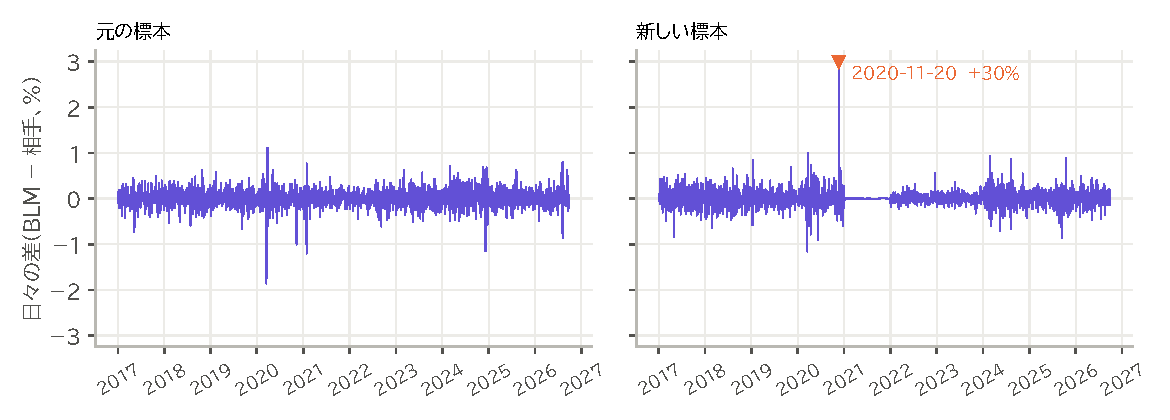
\includegraphics[width=\linewidth]{r1_active.pdf}
\caption{日々の差（BLM − 比べる相手、\%）。2017 年以降、四半期ごと、共分散 B、TE の校正あり。$\pm$3\% を超える日は端に印を付けた（『実験 R1』の図）。}
\label{fig:r1active}
\end{figure}

\section{誤りを除いた計算（探索）}

ありえない日々のリターンを欠けにして、S4 の主なポートフォリオを計算し直した。しきい値は計算の前に 3 通り決めた。しきい値なしの計算は S4 と完全に一致した。

\begin{table}[H]
\centering\small
\caption{誤りを除いた BLM（2015 年末から四半期ごと、ChronoGPT＋リッジ、共分散 B、TE の校正あり、2017 年以降 2,449 日）。}
\label{tab:explore}
\begin{tabular}{llrrrrrl}
\toprule
標本 & 日々のリターンの扱い & 除いた数 & $g$ & 実現の TE & 年の差 & 95\% 区間 & 片側 $p$ \\
\midrule
元 & そのまま & 0 & 1.05 & 3.2\% & +3.0\% & +1.2〜+5.0\% & 0.002 \\
元 & +300\%・$-80\%$ を除く（主） & 60 & 1.04 & 3.1\% & +3.0\% & +1.2〜+4.9\% & 0.0005 \\
新 & そのまま & 0 & 3.32 & 10.0\% & +5.3\% & +1.1〜+12.2\% & $<$ 0.0005 \\
新 & +300\%・$-80\%$ を除く（主） & 69 & 1.08 & 3.2\% & \textbf{+2.9\%} & +1.0〜+4.8\% & 0.0005 \\
新 & +100\%・$-50\%$ を除く & 417 & 1.07 & 3.2\% & +2.7\% & +0.8〜+4.5\% & 0.0015 \\
新 & +1000\%・$-90\%$ を除く & 25 & 1.06 & 3.2\% & +2.9\% & +1.0〜+4.8\% & $<$ 0.0005 \\
\bottomrule
\end{tabular}
\end{table}

\begin{itemize}
\item 誤りを除くと、新しい標本でも TE の校正は効いた（$g$ 1.24 → 1.08。元は 1.26 → 1.04）。
\item BLM は両方の標本で相手を年約 3\% 上回った。情報レシオは新しい標本で 0.89、元で 0.97。事前登録の値（年 +5.3\%）の約半分は、誤りによる上乗せだった。
\item しきい値を変えても、差は年 +2.7〜+2.9\% でほとんど変わらなかった。
\end{itemize}

\begin{figure}[H]
\centering
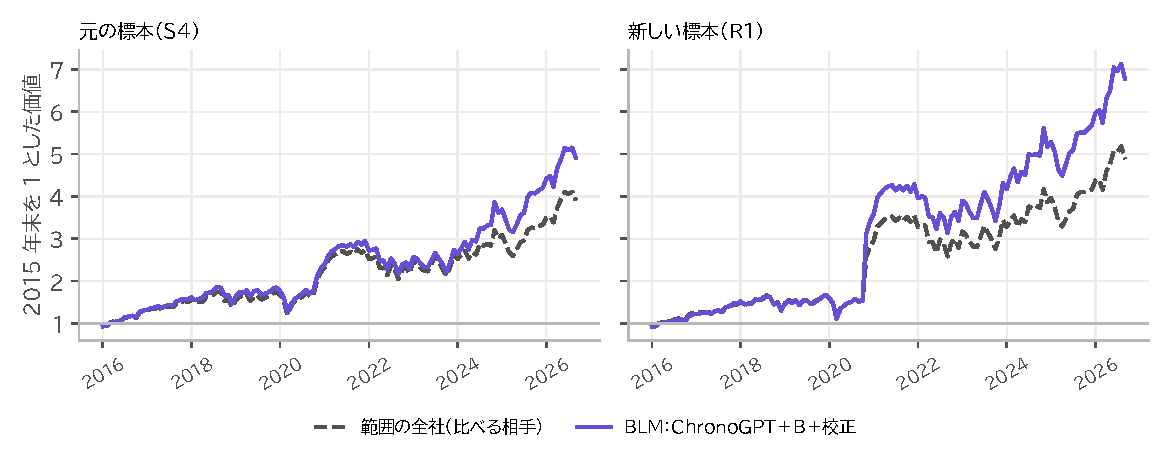
\includegraphics[width=\linewidth]{r1_paths.pdf}
\caption{2015 年末を 1 とした推移（誤りを除く前。『実験 R1』の図）。新しい標本の 2020 年 11 月の跳ね上がりの多くは、比べる相手にも BLM にも入っている株価の誤りである。}
\label{fig:r1paths}
\end{figure}

% ============================================================
\part{今どこまで言えるか}
% ============================================================

\chapter{結果の確かさ}\label{ch:status}

\section{3 つの問いに分ける}

「LLM の見通しを BLM に入れると役に立つか」は、3 つの問いに分かれる。それぞれの確かさは違う。

\begin{longtable}{p{5.0cm}p{2.8cm}p{6.0cm}}
\caption{問いごとの確かさ（2026-10-25 の時点）。}\label{tab:status}\\
\toprule
\textbf{問い} & \textbf{今の状態} & \textbf{根拠} \\
\midrule
\endfirsthead
\bottomrule
\endfoot
問い 1：決算発表文の読み取りに、小型株の値動きを予測する力があるか & \textbf{ほぼ確かめられた} & 事前登録した検定で支持され、重なりのない別の 1,000 社でも再現した（S1・S2） \\
問い 2：それを BLM に入れると、比べる相手に勝てるか & \textbf{有望だが、まだ証明ではない} & 両方の標本で年約 +3\%、片側 $p$ 0.0005（2,449 日）。ただし誤りを除いた数字は探索 \\
問い 3：勝った分は LLM の読み取りのおかげか & \textbf{まだ調べていない} & BLM の仕組みや、規模・割安さ・モメンタムへの傾きで勝った可能性を除いていない \\
\end{longtable}

\section{問い 2 がまだ証明でない理由}

\begin{itemize}
\item 事前登録した R-BLM の検定は「支持」だったが、その数字は株価の誤りに汚れていた。
\item 誤りを除いた +2.9\%・+3.0\% は、結果を見た後に「除こう」と決めた分析である。しきい値は計算の前に決めたが、事前登録の検定ではない。
\item 元の標本の BLM の数字（年 +3.0\%）は、R1 の事前登録より前に計算していた。
\end{itemize}

\section{弱点}

\begin{itemize}
\item \textbf{生存者バイアス}：今も株価がある会社だけを使っている。範囲の会社・年の 31.7\% が欠けている。
\item \textbf{費用と容量}：片道 0.3\% の一定で、売買による値の動き（市場への影響）を入れていない。
\item \textbf{同じ母集団・同じ期間}：新しい標本も、米国の小型株・2015〜2026 年の残りの会社である。
\item \textbf{単純なポートフォリオとのずれ}：上位 20\% の月次のポートフォリオは、両方の標本で有意でなかった（元 +0.16\%/月、$t$ 0.73。新 $-1.43\%$/月、$t$ $-0.88$）。
\end{itemize}

\section{中間発表で言えること}

\begin{keybox}[言い切ってよいこと]
\begin{itemize}
\item 小型株では、LLM で決算発表文を読んだ点数が、発表後 2〜60 日のドリフトを予測する。事前登録した検定で支持され、重なりのない別の 1,000 社でも再現した。
\item 発表後の変動率の予測も、両方の標本で再現した。
\item 主な分析には、先読みのない ChronoGPT を使った。
\item 大型株では、情報は発表の当日に株価に入っていた（小型株に移った理由）。
\end{itemize}
\end{keybox}

\begin{notebox}[条件をつけて言うこと・言わないこと]
\begin{itemize}
\item BLM は、株価の誤りを除くと、両方の標本で相手を年約 3\% 上回った（TE 約 3.2\%、情報レシオ約 0.9）。ただし探索の結果で、確かめる検定はこれから。
\item 事前登録した R-BLM の年 +5.3\% は、そのまま見せない。誤りを見つけて除いた過程を見せる。
\item 「BLM で勝てることが証明された」「実際の運用に使える」とは言わない。
\end{itemize}
\end{notebox}

\chapter{BLM が効くことの証明の計画}\label{ch:plan}

問い 2・3 を確かめるため、次の 6 つを計画した（リポジトリの \code{やること.md} の G）。順番は、G1・G2（今のデータで数時間）→ G4 の見積もり → G3 の事前登録（G1・G2・G5 を副次の検定として入れる）→ 1 回だけ実行、とする。G1・G2 の結果によっては G3 の計画を変える。

\begin{longtable}{p{0.8cm}p{6.4cm}p{6.6cm}}
\caption{証明のための確かめ。}\label{tab:plan}\\
\toprule
\textbf{\#} & \textbf{やること} & \textbf{理由} \\
\midrule
\endfirsthead
\toprule
\textbf{\#} & \textbf{やること} & \textbf{理由} \\
\midrule
\endhead
\bottomrule
\endfoot
G1 & \textbf{偽のビューとの比較}（探索）。各組み直しの日に、点数を銘柄の間で並べ替えた BLM を 100 回作る。共分散・$\Omega$・TE の校正・費用・誤りを除く規則は本物と同じ。本物の年約 +3\% が偽物の分布の上 5\% に入るかを、両方の標本で見る & BLM の仕組み（共分散の補正、TE の校正、相手との比率の違い）だけで勝っているなら、偽物も勝つ。大型株の実験 7・9 と同じ確かめ方 \\
G2 & \textbf{ファクターでの説明}（探索）。BLM と相手の日々の差を、Fama--French の 5 因子＋モメンタム（日次、2026-08-31 まで）に回帰し、$\alpha$ が残るかを見る。G1 の偽物の差も同じ回帰にかける & 規模・割安さ・モメンタムへの傾きで説明できるなら、読み取りの力とは言えない \\
G3 & \textbf{事前登録のやり直し}。誤りを除く規則（+300\% 超・$-80\%$ 未満の日々のリターンを欠けにする）、R-BLM の形、判定の基準を先にコミットで固定し、まだ使っていない会社で 1 回だけ検定する。残りは 400 社しかないので、先に検出力を見積もり、足りなければ G4 の上場廃止の会社を足す & 誤りのないデータの値を、事前登録した検定で確かめる \\
G4 & \textbf{生存者バイアス}。上場廃止の株価（EODHD など）を補えるかを確かめ、補えない分は、欠けた会社の扱いで結果がどこまで動くかを見積もる & 倒産した会社が抜けると、点数の低い会社の成績が良く見え、BLM の勝ちは控えめに出る（『小型株のデータ』の見立て）。上乗せ付きで買収された会社が抜ける影響は、点数の高低のどちらが買収されやすいかで向きが変わる \\
G5 & \textbf{費用と容量}。片道 0.5\%・1\% で計算し直し、売買の額が売買代金の何割かを出して、市場への影響（平方根の法則など）を足す & 小型株では費用が成績を決める \\
G6 & \textbf{単純なポートフォリオとのずれ}（探索）。上位 20\% のポートフォリオが有意でない理由を調べる & BLM の年 +3\% と食い違わないことを説明できないと、結論が弱い \\
\end{longtable}

\begin{keybox}[証明と言える条件]
G1 で本物が偽物の分布の上の端に来て、G2 で $\alpha$ が残り、G3 の事前登録した検定が誤りのないデータで支持され、G4・G5 で結論が覆らなければ、「小型株では、LLM の読み取りを BLM に入れると、比べる相手を上回る」と言える。
\end{keybox}

\chapter{この先の研究の形}\label{ch:future}

修士の 2 年まで続ける場合、この研究は次の 3 本の柱にできる。

\begin{enumerate}
\item \textbf{確かめる}：G1〜G6 を済ませてから事前登録し、修士の間に出る決算発表で 1 回だけ検定する。2026 年 11 月より後の発表は、まだ誰も見ていない。2 年で約 8 四半期、1,000 社でも約 8,000 本になる。前向きの検証は今は時間が足りないのでやめたが、修士の期間なら現実的である。また、これからの発表は新しいモデル（gpt-5.x など）の学習の期間より後なので、先読みを気にせずに強いモデルを使える。
\item \textbf{方法を作る}：LLM の点数を BLM にどう入れれば信号を失わないか。ビューの大きさを持つ期間に合わせること（X05）、$\Omega$（LLM の確信度）、TE の校正（S4）、共分散の補正（S3）。先行研究が手薄な部分で、この研究の独自性になる。
\item \textbf{広げる}（余裕があれば）：日本の小型株と決算短信。ただし、過去の決算短信の入手の方法と費用を先に確かめる必要がある。
\end{enumerate}

「LLM で決算の文章を読んで株価を当てる」研究は多い（Lopez-Lira・Tang 2023 など）。予測できることだけでは新しさが弱いので、「先読みのない読み取り」「小型株での再現」「BLM への正しい組み込み」の組み合わせで独自性を出す。

% ============================================================
\part{証明（G1〜G6 の結果）}
% ============================================================

\chapter{証明の結果}\label{ch:proof}

\begin{notebox}[この部は未完成]
この部は、\chapref{ch:plan} の G1〜G6 を行った後に書き足す。2026 年 10 月 25 日の時点では、どれもまだ行っていない。
\end{notebox}

% ============================================================
\part{まとめ}
% ============================================================

\chapter{道具と計算環境}\label{ch:tools}

\section{点数付けの計算}

ChronoGPT（1.55B）と FinBERT の点数付けは、手元の PC の GPU と、借りた GPU（RunPod、RTX 4090 を 2 枚）で行った。新しい標本の ChronoGPT の点数は、一部の発表を手元の PC でも付けて、借りた GPU の結果と一致することを確かめた。

\begin{table}[H]
\centering\small
\caption{小型株の費用。}
\label{tab:cost}
\begin{tabular}{lll}
\toprule
 & 元の標本 & 新しい標本（R1） \\
\midrule
gpt-4o-mini & 6.91 ドル（11,914 本） & 6.94 ドル（11,824 本、利用者が了承） \\
RunPod（ChronoGPT・FinBERT） & ― & 約 2.1 ドル \\
\bottomrule
\end{tabular}
\end{table}

\section{データベース}

小型株の DB（\code{data/smallcap.sqlite}、新しい標本は \code{data/smallcap\_rep.sqlite}、それぞれ約 1.1GB）は Git の外に置いた。DB・点数の保存先・結果のフォルダは環境変数で切り替えるので、同じコードで両方の標本を計算できる。

\section{読むためのコードの写し}

これまでのコードと設計を、段階ごとに 4 つのフォルダ（\code{工房/1\_元論文の再現/}、\code{2\_仮説の検証/}、\code{3\_大型株の決算発表/}、\code{4\_小型株と再現/}）に写し、日本語の注釈を付けた。各フォルダには、DB の接続（どのテーブルから何を読み、何を書くか）、LLM の接続、ロジック（BLM と最適化）、アーキテクチャの設計資料がある。関数の前には入力と出力を書いた。フォルダを分け直した写しなので、そのままでは動かない。

\chapter{結論}\label{ch:conclusion}

総合報告書 1 からの問い「LLM の見通しを Black--Litterman モデルに入れると、時価総額加重を上回るか」に、本書の作業は次のように答えた。

\begin{enumerate}
\item \textbf{大型株では上回らない。}LLM は決算発表文を読めるが（アナリスト予想・専用のモデル・先読みのない LLM を超える）、その情報は発表の当日に株価に入る。
\item \textbf{小型株では、読み取りが発表後のドリフトと変動率を予測する。}事前登録した検定で支持され、別の 1,000 社でも再現した。
\item \textbf{小型株の BLM は、株価の誤りを除くと、両方の標本で比べる相手を年約 3\% 上回った。}TE の校正も効いた。ただしこれは探索の結果で、証明ではない。
\end{enumerate}

次の一歩は、\chapref{ch:plan} の G1〜G6 である。偽のビューとファクターで「勝った分が読み取りから来たか」を確かめ、誤りを除く規則を先に固定して、まだ使っていないデータで 1 回だけ検定する。その結果は、本書の第 VI 部に書き足す。

\begin{keybox}[一言で]
LLM が決算発表文から読めることは、大型株では市場もその日のうちに読んでいるが、小型株では数か月かけて価格に入る。その読み取りを BLM に入れると、比べる相手を上回る見込みがある。ただし、その見込みを証明する確かめは、まだ残っている。
\end{keybox}

% ============================================================
\part{付録}
% ============================================================

\appendix

\chapter{主なコミット}\label{app:git}

すべてブランチ \code{feature/earnings-events} にあり、GitHub にプッシュ済み（強制プッシュはしていない）。

\begin{longtable}{p{1.6cm}p{1.6cm}p{10.6cm}}
\toprule
\textbf{日付} & \textbf{コミット} & \textbf{内容} \\
\midrule
\endfirsthead
\toprule
\textbf{日付} & \textbf{コミット} & \textbf{内容} \\
\midrule
\endhead
\bottomrule
\endfoot
10/18 & \code{97e80fa}、\code{11b6196} & X02〜X04 と報告書 \\
10/18 & \code{0ca1c1d} & 実験 7・8（月次と日次の BLM） \\
10/18 & \code{e7fdb15} & 実験 5（ChronoGPT の埋め込み＋リッジ） \\
10/19 & \code{807fe1f} & 実験 9（約 10 年の月次の BLM） \\
10/19 & \code{8a4e995} & 実験 10（ChronoGPT の LoRA） \\
10/19 & \code{35bddb8}、\code{98573b1} & X05（$\alpha$ の大きさ、探索） \\
10/19 & \code{17d05af} & 取り下げられた論文（Kim・Muhn・Nikolaev 2024）の引用を直した \\
10/21 & \code{ff35527}、\code{6591f06} & 実験 11 の結果と報告書 \\
10/21 & \code{52544c8} & 全体の記録（704 ページ） \\
10/23 & \code{e5af87c} & 小型株のデータと S1 の事前登録 \\
10/23 & \code{5f0e004} & S1 の追記 1（BLM の推移、反応を計算する前） \\
10/23 & \code{09427a4}、\code{69a0e12} & ヘッジファンドの手法の報告書、文献の照合 \\
10/24 & \code{188f2ce} & S1 の結果（支持） \\
10/24 & \code{ecf16bb}、\code{b70a755} & S2 の事前登録と結果（支持） \\
10/25 & \code{a6107fb}、\code{179491b} & S3 の事前登録と結果（支持されない） \\
10/25 & \code{1e027b6}、\code{c405858} & S4 の事前登録と結果（支持） \\
10/25 & \code{b08b9d0}、\code{161cab5} & R1 の標本と事前登録 \\
10/25 & \code{57245d0}〜\code{4a18414} & R1 の点数付け（gpt-4o-mini、RunPod の ChronoGPT・FinBERT） \\
10/25 & \code{08e238c}、\code{c6c988d} & R1 の結果・探索と報告書 \\
\end{longtable}

\chapter{資料の一覧}\label{app:docs}

\begin{longtable}{p{6.4cm}p{7.6cm}}
\toprule
\textbf{資料} & \textbf{中身} \\
\midrule
\endfirsthead
\bottomrule
\endfoot
\code{資料集/02\_実験/実験3\_アナリスト予想/}〜\code{実験11\_…/} & 大型株の実験 3〜5・7〜11 の報告書 \\
\code{資料集/02\_実験/補足実験\_共分散とTE/}、\code{補足実験\_}$\alpha$\code{の大きさ/} & X02〜X05 の報告書 \\
\code{資料集/02\_実験/小型株のデータ/} & 小型株の範囲、生存者バイアス、取得したデータ \\
\code{資料集/02\_実験/実験S1\_小型株のドリフト/}〜\code{実験S4\_TEの校正/} & S1〜S4 の報告書 \\
\code{資料集/02\_実験/実験R1\_新しい1000社での再現/} & R1 の報告書（再現、R-BLM、株価の誤りの探索） \\
\code{資料集/05\_解説/ヘッジファンドの投資手法/} & ヘッジファンドの投資手法の報告書（約 110 ページ） \\
\code{資料集/00\_全体の記録/} & 全体の記録（すべての資料を 1 冊にしたもの） \\
\code{設計\_小型株.md} & 小型株の設計 \\
\code{experiments/S1\_…/}〜\code{R1\_replication/} & 事前登録、コード、結果 \\
\code{やること.md} & 次にやることの一覧（G が証明の計画） \\
\end{longtable}

\chapter*{参考文献}
\addcontentsline{toc}{chapter}{参考文献}

\begin{itemize}\small
\item Bernard, V. L., Thomas, J. K. (1989). Post-Earnings-Announcement Drift: Delayed Price Response or Risk Premium? Journal of Accounting Research 27 (Supplement).
\item Black, F., Litterman, R. (1992). Global Portfolio Optimization. Financial Analysts Journal 48(5).
\item Chordia, T., Goyal, A., Sadka, G., Sadka, R., Shivakumar, L. (2009). Liquidity and the Post-Earnings-Announcement Drift. Financial Analysts Journal 65(4).
\item Fama, E. F., French, K. R. (2015). A Five-Factor Asset Pricing Model. Journal of Financial Economics 116(1).
\item Grinold, R. C. (1994). Alpha Is Volatility Times IC Times Score. Journal of Portfolio Management 20(4).
\item He, G., Litterman, R. (1999). The Intuition Behind Black-Litterman Model Portfolios. Goldman Sachs Investment Management Research.
\item He, S., Lv, L., Manela, A., Wu, J. (2025). Chronologically Consistent Large Language Models. arXiv:2502.21206.
\item Hong, H., Lim, T., Stein, J. C. (2000). Bad News Travels Slowly: Size, Analyst Coverage, and the Profitability of Momentum Strategies. Journal of Finance 55(1).
\item Huang, A. H., Wang, H., Yang, Y. (2023). FinBERT: A Large Language Model for Extracting Information from Financial Text. Contemporary Accounting Research 40(2).
\item Ledoit, O., Wolf, M. (2004). A Well-Conditioned Estimator for Large-Dimensional Covariance Matrices. Journal of Multivariate Analysis 88(2).
\item Lee, Y., Kim, Y., Kim, S., Lee, Y. (2025). LLM-Enhanced Black-Litterman Portfolio Optimization. arXiv:2504.14345.
\item Lopez-Lira, A., Tang, Y. (2023). Can ChatGPT Forecast Stock Price Movements? Return Predictability and Large Language Models. arXiv:2304.07619.
\item Martineau, C. (2022). Rest in Peace Post-Earnings Announcement Drift. Critical Finance Review 11(3--4).
\item Politis, D. N., Romano, J. P. (1992). A Circular Block-Resampling Procedure for Stationary Data. In: Exploring the Limits of Bootstrap, Wiley.
\end{itemize}

\end{document}
